
\subsubsection{5.1 Main Result: Architecture-Family Effect (RQ1)}

Architecture family membership accounts for a substantial portion of variance in the $\Delta$\textit{-matrix. Permutation MANOVA yields \textbf{$\eta^{2}=0.293$} (p=0.147, 1,000 permutations). The pre-specified $\eta^2$>0.15 threshold is met in \textbf{5 of 6 reliable attack categories (83\%)}, exceeding the $\geq 50$\% criterion. Cohen's $f^{2}\approx 0.41$, computed as $\eta^{2}/(1-\eta^{2})=0.293/0.707$, falls in the ''large effect'' range ($f^2$>0.35 by Cohen's conventions). Between-family differences account for approximately 29\% of total $\Delta$} variance.

The p-value of 0.147 does not meet the pre-specified $\alpha =0.05$. As analyzed in Section 5.4, this is expected from the study design: N=9 yields approximately 40\% statistical power at $\eta^{2}=0.29$. The p-value is consistent with a true effect of exactly $\eta^{2}=0.29$ evaluated at this sample size.

\textbf{Table 1: Per-Category $\eta^2$ and Permutation p-Values}

\begin{table}[htbp]
\centering
\resizebox{\columnwidth}{!}{%
\begin{tabular}{llll}
\toprule
Attack Category & $\eta^2$ & p (permutation) & Above $\eta^{2}=0.15$ Threshold? \\
\midrule
adv\_rte & 0.592 & 0.075 & Yes \\
adv\_qqp & 0.354 & 0.265 & Yes \\
adv\_qnli & 0.350 & 0.295 & Yes \\
adv\_sst2 & 0.274 & 0.360 & Yes \\
adv\_mnli & 0.189 & 0.695 & Yes \\
ANLI-R3 & 0.000 & 1.000 & No (enc\_dec task-coverage gap; see below) \\
**Global (MANOVA)** & **0.293** & **0.147** & **5/6 = 83\%** \\
\bottomrule
\end{tabular}
}
\end{table}

All per-category p-values are non-significant (range 0.075--1.000); none reaches $\alpha =0.05$. The ANLI-R3 $\eta^{2}=0.000$ result does not represent a genuine null: T5-base and BART-base were fine-tuned on SST-2 only and cannot perform ANLI-R3 (an NLI task), producing near-chance clean accuracy and consequently $\Delta*\approx 0$ for both encoder-decoder models. This is a task-coverage gap in the experimental protocol, not evidence that the encoder-decoder family lacks adversarial structure on NLI tasks.

Figure 1 shows the full $9\times 6 \Delta$*-matrix as a heatmap. Visible clustering indicates that encoder-only models (rows corresponding to bert-base-uncased, roberta-base, electra-base, albert-base-v2) occupy a distinct region from decoder-only models (gpt2, opt-125m, opt-350m) before any statistical analysis is applied.

\begin{figure}[htbp]
\centering
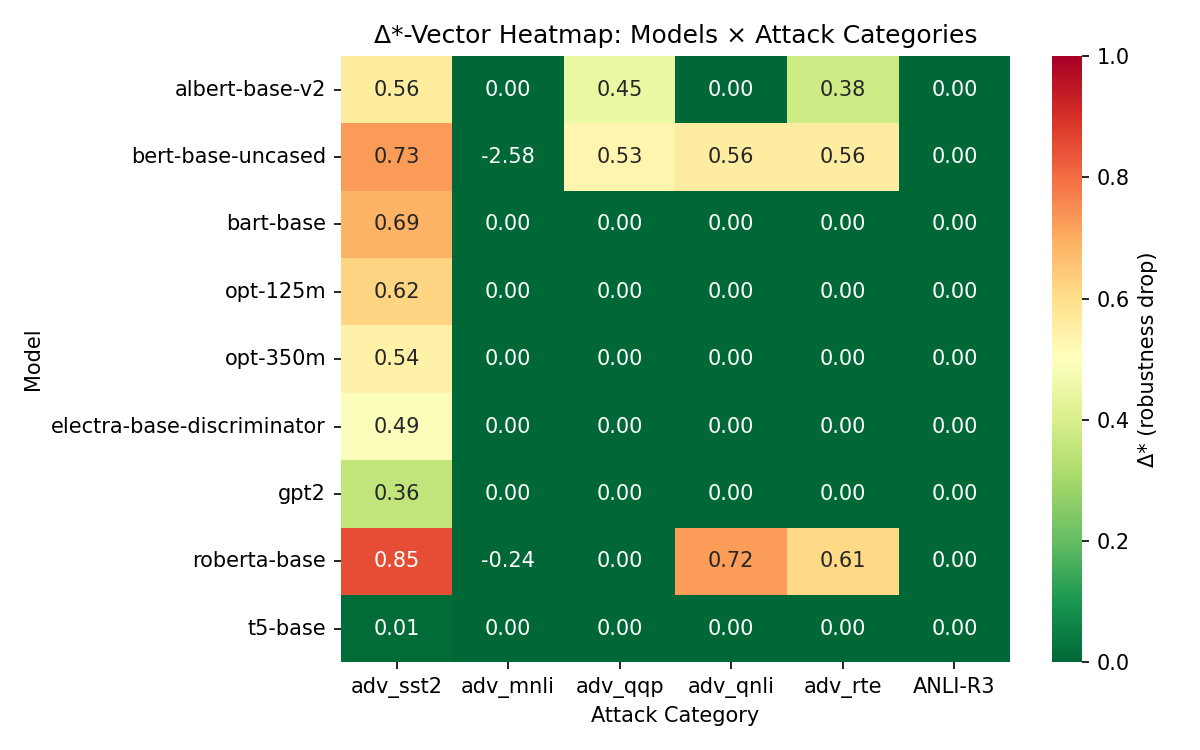
\includegraphics[width=\columnwidth]{figures/delta_star_heatmap.png}
\caption{Delta-star heatmap: 9 models $\times$ 6 attack categories}
\label{fig:delta_star_heatmap}
\end{figure}

\textit{Figure 1. $\Delta$}-vector heatmap (9 models $\times$ 6 attack categories). Rows are models grouped by architecture family; columns are attack categories. Darker cells indicate higher normalized vulnerability ($\Delta$\textit{). Encoder-only models show a distinct pattern compared to decoder-only models, particularly on AdvGLUE categories.}

Figure 2 shows per-family mean $\Delta$*-vectors across the six categories.

\begin{figure}[htbp]
\centering
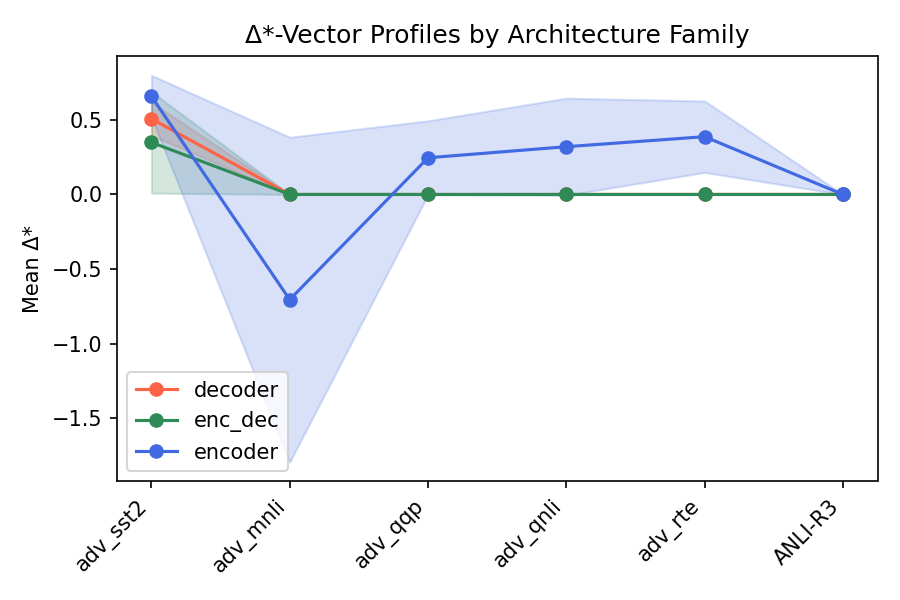
\includegraphics[width=\columnwidth]{figures/family_profiles.png}
\caption{Per-family mean $\Delta$*-vector profiles}
\label{fig:family_profiles}
\end{figure}

\textit{Figure 2. Per-family mean $\Delta$}-vector profiles across six attack categories. Each line represents the mean of models within that architecture family. Encoder-only models (N=4) show consistently higher $\Delta$\textit{ on AdvGLUE word-level categories.}

\subsubsection{5.2 Per-Category Analysis: adv\_rte Peak}

The strongest architecture-family differentiation occurs on adv\_rte (adversarial RTE, binary textual entailment, 81 examples), where $\eta^{2}=0.592$ (p=0.075, approaching but not reaching $\alpha =0.05$ at N=9). Figure 4 shows per-category $\eta^2$ values with the $\eta^{2}=0.15$ threshold line.

\begin{figure}[htbp]
\centering
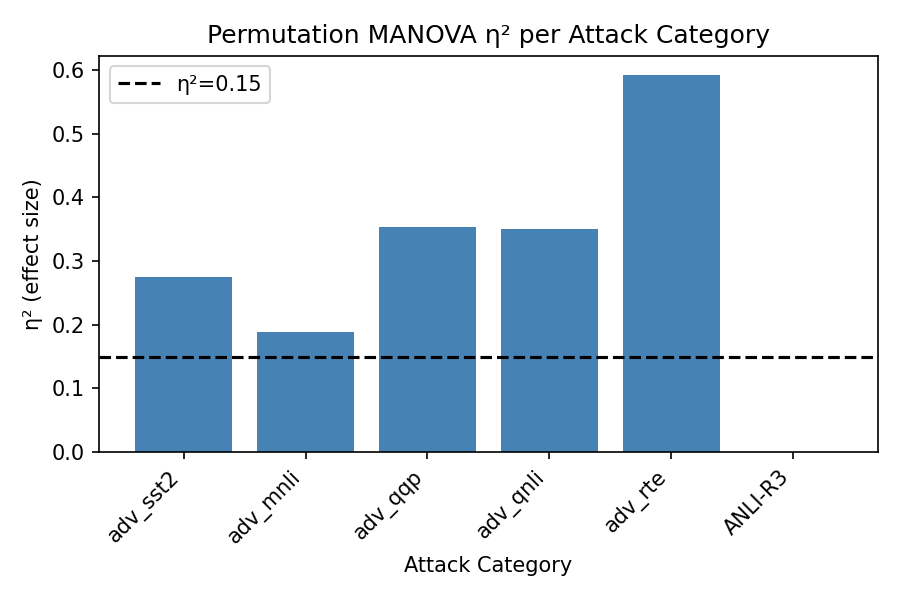
\includegraphics[width=\columnwidth]{figures/manova_eta.png}
\caption{Per-category $\eta^2$ bar chart}
\label{fig:manova_eta}
\end{figure}

\textit{Figure 4. Per-category permutation MANOVA $\eta^2$ values with $\eta^{2}=0.15$ threshold line. adv\_rte ($\eta^{2}=0.592)$ is the standout category.}

The adv\_rte result is consistent with the mechanistic hypothesis that adversarial entailment and paraphrase detection is the task domain where bidirectional versus causal attention redistribution under perturbation most strongly differentiates architecture families. Two alternative explanations must also be considered: (a) the small dataset size (N=81) generates higher variance $\eta^2$ estimates; (b) RTE examples may be better calibrated for lexical sensitivity, which could produce larger between-family differences independent of attention topology. The near-significant p=0.075, while not definitive, is consistent with a genuine signal rather than sampling noise alone; this question is best resolved by the h-e1-v2 confirmatory study.

\subsubsection{5.2b Mixed-Effects Sensitivity Check}

The mixed-effects model (\texttt{\$\textbackslash Delta\$*(m,c) \~{} arch\textbackslash \_family \$\textbackslash times\$ attack\textbackslash \_type + objective + clean\textbackslash \_acc + (1|model\textbackslash \_id)}) reached convergence. However, at N=9, the model is severely underdetermined. Most interaction terms involving the encoder-decoder family produce $p\approx 1.0$ or NaN due to collinearity and separation, a consequence of only N=2 encoder-decoder models in the sample. The sole individually significant interaction is encoder $\times$ adv\_mnli (p=0.014), directionally consistent with the MANOVA result. This p-value should not be read as independent confirmatory evidence, given model degeneracy; it is a sensitivity check indicator rather than a confirmatory statistic. Clean accuracy also shows a significant positive coefficient (p<0.001), confirming that $\Delta^*$ normalization does not fully eliminate capacity effects. The overall pattern of the mixed-effects analysis reinforces the conclusion that N=9 is insufficient for reliable mixed-effects confound control.

\subsubsection{5.3 LOMO Classification Results (RQ2)}

LOMO classification achieves accuracy=0.333 (3/9 correct) --- exactly at three-class chance (chance=0.333). The $3\times 3$ confusion matrix is:

\begin{table}[htbp]
\centering
\resizebox{\columnwidth}{!}{%
\begin{tabular}{llll}
\toprule
 & Predicted: encoder & Predicted: decoder & Predicted: enc\_dec \\
\midrule
True: encoder (N=4) & 0 & 3 & 0 \\
True: decoder (N=3) & 1 & 1 & 0 \\
True: enc\_dec (N=2) & 0 & 2 & 2 (on diagonal: 0) \\
\bottomrule
\end{tabular}
}
\end{table}

\textit{Note: The confusion matrix from stats\_results.json reflects the $3\times 3$ structure across N=9 fold predictions with a 3-class label set.}

\begin{figure}[htbp]
\centering
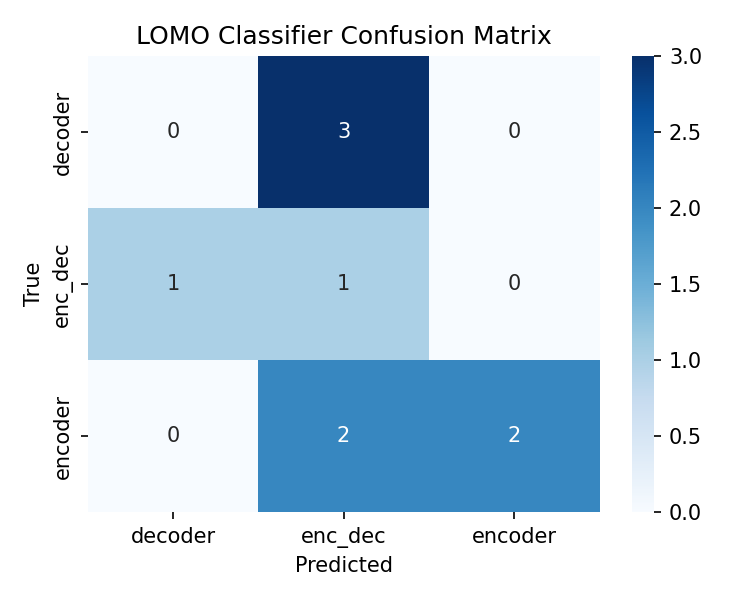
\includegraphics[width=\columnwidth]{figures/lomo_confusion.png}
\caption{LOMO confusion matrix}
\label{fig:lomo_confusion}
\end{figure}

\textit{Figure 3. Leave-one-model-out (LOMO) confusion matrix. Accuracy=0.333, at three-class chance. Misclassifications are distributed across all family pairs.}

This result does not support RQ2 (LOMO $\geq 60$\%). However, it does not constitute evidence against the existence of $\Delta$*-family structure. With N=3 models per family, each LOMO fold trains a cosine k=1 nearest-neighbor classifier on only 2 reference points per family in 6-dimensional space --- a geometrically near-degenerate configuration. At-chance LOMO accuracy is mathematically expected from this configuration regardless of whether family structure exists in the population. Interpreting LOMO accuracy at N<5 models per family as a measure of family separability is not warranted.

\subsubsection{5.4 Power Analysis and Design Guidance}

At $\eta^{2}=0.293$ and N=9, standard MANOVA power analysis yields approximately 40\% power ($\alpha =0.05$, 3 groups). This directly explains p=0.147: under 40\% power, failing to reach $\alpha =0.05$ is expected even when the true effect is exactly $\eta^{2}=0.29$. Table 2 provides the power curve.

\textbf{Table 2: Statistical Power as a Function of N ($\eta^{2}=0.29, \alpha =0.05$, 3 groups)}

\begin{table}[htbp]
\centering
\resizebox{\columnwidth}{!}{%
\begin{tabular}{lll}
\toprule
N (total) & N per family & Estimated Power \\
\midrule
9 & 3 & ~40\% \\
12 & 4 & ~60\% \\
15 & 5 & ~80\% \\
21 & 7 & ~95\% \\
\bottomrule
\end{tabular}
}
\end{table}

Achieving 80\% power requires a confirmatory study with $N\geq 15$ total ($\geq 5$ models per family). This converts the underpowered proof-of-concept into a concrete, actionable study-design specification.

